\documentclass{article}

%%% Packages %%%

% Graphics
\usepackage{graphicx}
\usepackage[caption=false,font=footnotesize]{subfig}

% Formatting
\usepackage{color}
\usepackage{amsmath}
\usepackage{amsfonts}
\usepackage{bbm}
\usepackage[T1]{fontenc}

% Environments
\usepackage{IEEEtrantools}
\usepackage{algorithm}
\usepackage{algorithmic}

% References
\usepackage{natbib}

\graphicspath{{figures/}}

%%% Macros %%%
%%% MACROS FOR MATHEMATICAL NOTATION IN COMPOSITE PROPOSAL PAPER %%%

% Functions and operators
\newcommand{\half}{\frac{1}{2}}                                 % Half
\newcommand{\expect}[1]{\mathbb{E}_{#1}}                        % Expectation
\newcommand{\variance}[1]{\mathbb{V}_{#1}}                      % Variance
\DeclareMathOperator{\trace}{Tr}                                % Trace
\newcommand{\magdet}[1]{\left| #1 \right|}         % Magnitude of the determinant
\newcommand{\indic}[1]{\mathbbm{1}_{#1}}                        % Indicator function
\newcommand{\normal}[3]{\mathcal{N}\left(#1\left|#2,#3\right.\right)}       % Normal density
\newcommand{\gammaden}[3]{\mathcal{\Gamma}\left(#1|#2,#3\right)}% Gamma density
\newcommand{\studentt}[4]{\mathcal{ST}\left(#1|#2,#3,#4\right)} % Student-t density
\newcommand{\bigo}[1]{\mathcal{O}\left({#1}\right)}             % Big O
\newcommand{\mhaccept}{\alpha}                                  % Metropolis-Hastings acceptance probability

% Basics
\newcommand{\rt}{t}                             % Real time
\newcommand{\pt}{\lambda}                       % Pseudo-time
\newcommand{\dpt}{\delta\lambda}                % A little bit of pseudo-time
\newcommand{\ls}[1]{x_{#1}}                     % Latent state
\newcommand{\ob}[1]{y_{#1}}                     % Observation
\newcommand{\mix}[1]{\xi_{#1}}                  % Mixing auxiliary variable
\newcommand{\els}[1]{u_{#1}}                    % Extra latent state

% Particle shizzle
\newcommand{\pss}[2][]{^{(#2)#1}}               % Particle superscript
\newcommand{\pw}[1]{w_{#1}}                     % Particle weight
\newcommand{\predpw}[1]{\hat{w}_{#1}}           % Predictive particle weight
\newcommand{\npw}[1]{\bar{w}_{#1}}              % Normalised particle weight
\newcommand{\naw}[1]{\bar{v}_{#1}}              % Normalised auxiliary weight
\newcommand{\anc}[1]{a_{#1}}                    % Particle ancestor

% Densities
\newcommand{\transden}{f}                       % Transition density
\newcommand{\obsden}{g}                         % Observation density
\newcommand{\impden}{q}                         % Importance density
\newcommand{\partden}{\eta}                     % Unweighted particle distribution
\newcommand{\artden}{\rho}                      % Artificial conditional density
\newcommand{\oiden}[1]{\pi_{#1}}                % Optimal importance density
\newcommand{\approxoiden}[2]{\hat{\pi}_{#1|#2}} % Approximation of the optimal importance density
\newcommand{\augfiltden}[1]{\tilde{\pi}_{#1}}   % Augmented filtering density
\newcommand{\oinorm}[1]{K_{#1}}                 % Normalising constant for the optimal importance density
\newcommand{\augfiltnorm}[1]{\tilde{K}_{#1}}    % Normalising constant for the augmented filtering density

% Numbers
\newcommand{\numpart}{N_F}                      % Number of filter particles
\newcommand{\ess}[1]{N_{E,#1}}                  % Effective sample size

% Models
\newcommand{\transfun}{\phi}                    % Transition function
\newcommand{\obsfun}{h}                         % Observation function
\newcommand{\transcov}{Q}                       % Transition covariance
\newcommand{\obscov}{R}                         % Observation covariance
\newcommand{\transmat}{F}                       % Linear transition matrix
\newcommand{\obsmat}{H}                         % Linear observation matrix
\newcommand{\transmean}{m}                      % Mean of the transition density (i.e. f(x_{t-1}))
\newcommand{\dof}{\nu}                          % Degrees of freedom of something student-t-ish

% Linear Gaussian things
\newcommand{\lgoimean}[1]{\mu_{#1}}             % Linear Gaussian optimal importance density mean
\newcommand{\lgoicov}[1]{\Sigma_{#1}}           % Linear Gaussian optimal importance density covariance
\newcommand{\stdnorm}[1]{z_{#1}}                % Standard normal R.V.

% Gaussian Transformation
\newcommand{\lgdecayfunc}{a}                    % Linear Gaussian decay function for OID transformation
\newcommand{\lgexpsf}{\gamma}                   % Linear Gaussian exponential scale factor for OID transformation
\newcommand{\lgupdmeanmat}[1]{\Gamma_{#1}}      % Mean mapping matrix for the OID transformation
\newcommand{\lgupdcov}[1]{\Omega_{#1}}          % Covariance matrix for the OID transformation
\newcommand{\lginfbm}[1]{\epsilon_{#1}}         % Brownian motion for the infinitesimal form of the OID transformation

% Linear Gaussian approximations
%\newcommand{\lgoimeanapprox}[2]{\hat{\mu}_{#1}(#2)}     % Mean of the Gaussian approximation to the OID at time #1 and state #2
%\newcommand{\lgoicovapprox}[2]{\hat{\Sigma}_{#1}(#2)}   % Covariance of the Gaussian approximation to the OID at time #1 and state #2
\newcommand{\lgoimeanapprox}[2]{\hat{\mu}_{#1|#2}}      % Mean of the Gaussian approximation to the OID at time #1 and state #2
\newcommand{\lgoicovapprox}[2]{\hat{\Sigma}_{#1|#2}}    % Covariance of the Gaussian approximation to the OID at time #1 and state #2
\newcommand{\obsmatapprox}[1]{\hat{\obsmat}_{#1}}       % Linear observation matrix formed by differentiation of the observation function
\newcommand{\transmeanapprox}[1]{\hat{\transmean}_{#1}} % Approximate transition mean
\newcommand{\transcovapprox}[1]{\hat{\transcov}_{#1}}   % Approximate transition covariance
\newcommand{\obapprox}[1]{\hat{y}_{#1}}                 % Approximate observation mean
\newcommand{\obscovapprox}[1]{\hat{\obscov}_{#1}}       % Approximate observation covariance
\newcommand{\lsfixed}{\ls{}^*}                          % Latent state around which we linearise
\newcommand{\logtrans}{L}                               % Log of the transition density
\newcommand{\logobs}{M}                                 % Log of the observation density

% State evolution SDE
\newcommand{\oudrift}[1]{A_{#1}}                % General O-U process drift term
\newcommand{\oudiffuse}[1]{B_{#1}}              % General O-U process diffusion term
\newcommand{\sdedrift}[1]{\zeta_{#1}}           % Drift
\newcommand{\lserror}[2]{e_{#1|#2}}             % State error due to finite sampling

% Particle flow
\newcommand{\flowbm}[1]{\epsilon_{#1}}          % Particle flow Brownian motion
\newcommand{\flowdrift}[1]{\zeta_{#1}}          % Particle flow drift
\newcommand{\flowdiffuse}[1]{\eta_{#1}}         % Particle flow diffusion
\newcommand{\flowcov}[1]{D_{#1}}                % Particle flow "Covariance" matrix
\newcommand{\flowtd}{\alpha}                    % Flow dervation transition density
\newcommand{\flowod}{\beta}                     % Flow derivation observation density

% Simulation models - tracking
\newcommand{\pos}[1]{p_{#1}}           % Position
\newcommand{\vel}[1]{v_{#1}}           % Velocity
\newcommand{\bng}[1]{\theta_{#1}}               % Bearing
\newcommand{\rng}[1]{r_{#1}}                    % Range
\newcommand{\hei}[1]{h_{#1}}                    % Height
\newcommand{\rngrt}[1]{s_{#1}}                  % Range rate
\newcommand{\terrain}{T}                        % Terrain height

% Simulation models - heartbeats
\newcommand{\amp}[1]{A_{#1}}                    % Amplitude
\newcommand{\wid}[1]{W_{#1}}                    % Width
\newcommand{\del}[1]{\tau_{#1}}                 % Delay
\newcommand{\freq}[1]{\omega_{#1}}              % Width
\newcommand{\pha}[1]{\psi_{#1}}                 % Phase
\newcommand{\bias}[1]{B_{#1}}                   % Bias





%%% Environments %%%
\newenvironment{meta}[0]{\color{red} \em}{}
\newtheorem{lemma}{Lemma}



%%% Titles and stuff %%%
%\title[Composite Proposal Particle Filter]{The Composite Proposal Particle Filter: Better Approximations to the Optimal Importance Density}
%\author[Bunch {\it et al.}]{Pete Bunch}
%\address{Cambridge University Engineering Department,Cambridge,UK.}
%\email{pb404@cam.ac.uk}
\title{The Composite Proposal Particle Filter: Better Approximations to the Optimal Importance Density}
\author{Pete Bunch}



%%% DOCUMENT %%%

\begin{document}

\maketitle

\begin{abstract}
Abstract here.
\end{abstract}



%\keywords{particle filter, sequential Monte Carlo, optimal importance distribution}



\section{Introduction}

A particle filter is an algorithm used for sequential inference of a filtering distribution associated with a hidden Markov state-space model. The particle filter advances a set of samples through time, drawn approximately from the filtering distribution. This is achieved by sampling at each time step from an importance distribution and then weighting the particles to account for the discrepancy between filtering and importance distributions. Particle filters have attractive asymptotic properties: as the number of particles is increased, certain estimates are guaranteed to converge to their true values. For a comprehensive introduction, see for example \citep{Cappe2007,Doucet2009}.

One of the principal difficulties when designing a particle filter is the selection of the importance distribution. The simplest choice is often to sample from the transition model, resulting in the ``bootstrap filter'' of \citep{Gordon1993}. In many cases, such bootstrap proposals result in poor filter performance due to a mismatch in the areas of high probability between the transition and observation distributions.

Amongst others, \citet{Doucet2000a} demonstrated that the ideal choice of importance distribution for each particle is the conditional posterior given both the previous state and the new observation, dubbed the ``optimal importance distribution'' (OID). In all but a few cases, this cannot be calculated analytically. When the state variables are continuous, a popular solution is to use linearisation or the unscented transform to select a Gaussian importance density which approximates the OID for each particle \cite{Doucet2000a,Merwe2000}. However, such schemes can fail when the model is highly nonlinear or non-Gaussian, as the approximation is poor.

The effect of using a bad importance distribution (i.e. one which is not ``close'' to the OID) is that the variance of the importance weights is high, resulting in a degeneracy of the filter. In the worst cases, there may be no particles at all proposed in regions of high posterior probability, causing the filter to fail entirely. This problem is especially pronounced when the dimensionality of the state space is high --- there is simply more space for the particles to cover.
%
%Numerous additions and modifications to the basic particle filter have been proposed. For example, with some models it may be possible to marginalise a subset of the state variables --- a process known as ``Rao-Blackwellisation'' --- and hence to reduce the dimensionality of the samples in the particle filter \citep{Casella1996,Doucet2000}.

A common enhancement to the basic particle filter, which helps to alleviate the problems of degeneracy, is to include Markov chain Monte Carlo (MCMC) steps in order to rejuvenate a degenerate set of particles, a method named ``resample-move'' by \citet{Gilks2001}. When the importance sampling step has resulted in only a few useful particles in high probability areas, MCMC steps allow copies of these to be perturbed, so that they become better spread over the state space while still maintaining the correct distribution. While resample-move can often provide a useful fix for a struggling particle filter, it would be preferable to improve the initial importance sampling step to that such a fix is not required. There is, after all, a limit to what resample-move can practically achieve; if the importance sampling fails to put any particles in the right areas then a very large number of MCMC steps may be needed to get them there. In addition, an MCMC stage introduces new algorithm parameters which need to be tuned for effective operation, e.g. the number of MCMC steps per particle, and the proposal distribution.

Another way in which degeneracy may be mitigated is by introducing the effect of each observation gradually, so that particles may be progressively drawn towards peaks in the likelihood. This can be achieved by using a discrete set of bridging distributions which transition smoothly between the prior and posterior. Each one is targeted in turn using importance sampling and particle diversity is maintained using Metropolis-Hastings moves. Such ``annealing'' schemes have been suggested by, amongst others, \citet{Neal2001} (using MCMC) and \citet{DelMoral2006} (using Sequential Monte Carlo (SMC) samplers) for static inference problems, and by \citet{Godsill2001b,Gall2007,Deutscher2000} for particle filters.

It is possible to take the idea of bridging distributions to a limit and define a continuous sequence of distributions between the prior and the posterior. This device was used by \citet{Gelman1998} for the related task of simulating normalising constants, and has been used to design sophisticated assumed density filters \citep{Hanebeck2003a,Hanebeck2012,Hagmar2011}. More recently, particle filters have appeared which exploit the same principle, including the ``particle flow'' methods described in series of papers including \citep{Daum2008,Daum2011d}, and the ``optimal transport'' methods of \cite{Reich2011,Reich2012a}.

\subsection{Composite Proposals}

In this paper, a new method is introduced for sampling from an approximation of the optimal importance density; we name the resulting algorithm the composite proposal particle filter (CPPF). The objective of the composite proposal method is to provide a more efficient particle filter for challenging problems, on which standard particle filters fail. In common with progressive filtering and particle flow algorithms, the procedure relies on introducing the observation likelihood gradually. Beginning with a sample from the transition density, a series of updates using local approximations are then used to move the particle to a new state, either deterministically or stochastically. This method is shown to yield significant improvements in effective sample size for challenging nonlinear models.

%A modification of the algorithm is also presented which introduces intermediate resampling steps during the smooth update. This helps further to limit degeneracy of the particle weights, at the cost of introducing dependency between the particles. This latter algorithm resembles (and yet is significantly different from) an annealed particle filter \citep{Gall2007,Deutscher2000}, but uses gradient information from the model densities to lead particles towards peaks in the OID. In this sense, there are also connections with adaptive MCMC methods, such as those of \citep{Girolami2011}.



\section{Particle Filtering}\label{sec:pf}

We consider a standard discrete-time HMM in which the transition, observation and prior models have closed-form densities,
%
\begin{IEEEeqnarray}{rCl}
 \ls{\rt} & \sim & \transden(\ls{\rt} | \ls{\rt-1}) \label{eq:td} \\
 \ob{\rt} & \sim & \obsden(\ob{\rt} | \ls{\rt})   \label{eq:od} \\
 \ls{1} & \sim & p(\ls{1})                  \label{eq:pd}      ,
\end{IEEEeqnarray}
%
where the random variable $\ls{\rt}$ is the hidden state of a system at time $\rt$, and $\ob{\rt}$ is an incomplete, noisy observation. We assume here that the transition, observation and prior densities may be evaluated and that the prior and transition densities may be sampled. A particle filter is used to estimate recursively distributions over the path of the state variables, $\ls{1:\rt}=\{\ls{1}, \dots, \ls{\rt}\}$. Densities are approximated by a sum of weighted probability masses located at a discrete set of states,
%
\begin{IEEEeqnarray}{rCl}
 p(\ls{1:\rt} | \ob{1:\rt}) & = & \sum_i \npw{\rt}\pss{i} \delta_{\ls{1:\rt}\pss{i}}(\ls{1:\rt})     ,
\end{IEEEeqnarray}
%
where $\delta_{\ls{1:\rt}\pss{i}}(\ls{1:\rt})$ denotes a unit probability mass at the point $\ls{1:\rt}\pss{i}$ and the weight sum to $1$.

Particle filters have the highly desirable property of asymptotic consistency; as the number of particles tends to infinite, integrals of bounded functions over the filtering density converge to the true value,
%
\begin{IEEEeqnarray}{rCl}
 \sum_i \npw{\rt}\pss{i} \phi(\ls{1:\rt}\pss{i}) \rightarrow \int p(\ls{1:\rt}|\ob{1:\rt}) \phi(\ls{1:\rt}) d\ls{1:\rt}     \nonumber .
\end{IEEEeqnarray}

The particle filter recursion may be separated into two stages --- prediction and update --- which produce approximations to the predictive density, $p(\ls{1:\rt} | \ob{1:\rt-1})$, and filtering density, $p(\ls{1:\rt} | \ob{1:\rt})$, respectively. (Note, these terms more conventionally refer to the density of the latest state only, rather than the entire path.)

\subsection{The Algorithm}

For a simple particle filter (in which resampling is not optional and auxiliary sampling is not used), the prediction stage at time $\rt$ begins with selection (resampling) of a parent from amongst the $\rt-1$ particles; an index, $\anc{j}$, is chosen with probability $\npw{t-1}\pss{j}$. This selected particle trajectory $\ls{\rt_{1:t-1}}\pss{\anc{j}}$ is then approximately distributed according to $p(\ls{1:\rt-1}|\ob{1:\rt-1})$. Next, a new state $\ls{\rt}\pss{j}$ is sampled from an importance density, $\impden(\ls{\rt} | \ls{\rt-1}\pss{\anc{j}}, \ob{\rt})$, and concatenated to the parent path to form the new particle,
%
\begin{IEEEeqnarray}{rCl}
 \ls{1:\rt}\pss{j} \leftarrow \left\{ \ls{1:\rt-1}\pss{\anc{j}},  \ls{\rt}\pss{j} \right\}     .
\end{IEEEeqnarray}
%
An importance weight is then assigned to the particle to account for the discrepancy between importance and target distributions,
%
\begin{IEEEeqnarray}{rCl}
 \predpw{\rt}\pss{j} & = & \frac{ p(\ls{1:\rt}\pss{j} | \ob{1:\rt-1}) }{ p(\ls{1:\rt-1}\pss{\anc{j}} | \ob{1:\rt-1}) \impden(\ls{\rt}\pss{j} | \ls{\rt-1}\pss{\anc{j}}, \ob{\rt}) } \nonumber \\
 & \propto & \frac{ \transden(\ls{\rt}\pss{j} | \ls{\rt-1}\pss{\anc{j}}) }{ \impden(\ls{\rt}\pss{j} | \ls{\rt-1}\pss{\anc{j}}, \ob{\rt}) }     .
\end{IEEEeqnarray}

In the update stage, the same set of particles is used to approximate the filtering distribution. Since these are currently distributed according to,
%
\begin{IEEEeqnarray}{rCl}
 p(\ls{1:\rt-1} | \ob{1:\rt-1}) \impden(\ls{\rt} | \ls{\rt-1}, \ob{\rt}) \nonumber      ,
\end{IEEEeqnarray}
%
a new importance weight is required to account for the discrepancy,
%
\begin{IEEEeqnarray}{rCl}
 \pw{\rt}\pss{j} & = & \frac{ p(\ls{1:\rt}\pss{j} | \ob{1:\rt}) }{ p(\ls{1:\rt-1} | \ob{1:\rt-1}) \impden(\ls{\rt} | \ls{\rt-1}, \ob{\rt}) } \nonumber \\
 & \propto & \predpw{\rt}\pss{j} \times \obsden(\ob{\rt} | \ls{\rt}\pss{j} ) \nonumber       .
\end{IEEEeqnarray}

Finally, the weights are normalised,
%
\begin{IEEEeqnarray}{rCl}
 \npw{\rt} & = & \frac{ \pw{\rt}\pss{j} }{ \sum_i \pw{\rt}\pss{i} }      .
\end{IEEEeqnarray}

If the two steps are considered together, then the combined weight update is,
%
\begin{IEEEeqnarray}{rCl}
 \pw{\rt}\pss{j} & = & \frac{ p(\ls{1:\rt}\pss{j} | \ob{1:\rt}) }{ p(\ls{1:\rt-1}\pss{\anc{j}} | \ob{1:\rt-1}) \impden(\ls{\rt}\pss{j} | \ls{\rt-1}\pss{\anc{j}}, \ob{\rt}) } \nonumber \\
 & \propto & \frac{ \obsden(\ob{\rt} | \ls{\rt}\pss{j}) \transden(\ls{\rt}\pss{j} | \ls{\rt-1}\pss{\anc{j}}) }{ \impden(\ls{\rt}\pss{j} | \ls{\rt-1}\pss{\anc{j}}, \ob{\rt}) }     .
\end{IEEEeqnarray}

\subsection{Performance and Importance Distributions}

The practical performance of the particle filter is determined by the variance of the weights. An inefficient filter will suffer from high weight variance, meaning that only a small proportion of the particles (perhaps only one) is significant, and only these will be taken forward to the next filtering step. Clearly, fewer significant particles leads to a poorer representation of the distribution, resulting in increased estimator variance and propensity for the filter to diverge completely from the true distribution. The particle weight variance may be measured using the effective sample size (ESS), defined as,
%
\begin{IEEEeqnarray}{rCl}
 \ess{\rt} & = & \frac{ 1 }{ \sum_i \npw{\rt}\pss[2]{i} }     ,
\end{IEEEeqnarray}
%
Intuitively, this is the number of particles which would be present in an equivalent set comprised of independent, unweighted samples. It takes a value between $1$ (which is bad) and the number of filtering particles, $\numpart$ (which is good).

An essential consideration when designing a particle filter is the choice of importance density. The simplest option is to use the transition density,
%
\begin{IEEEeqnarray}{rCl}
 \impden(\ls{\rt} | \ls{\rt-1}\pss{\anc{j}}, \ob{\rt}) = \transden(\ls{\rt} | \ls{\rt-1}\pss{\anc{j}})     .
\end{IEEEeqnarray}
%
This results in the ``bootstrap filter'' of \cite{Gordon1993}. It only requires that sampling be possible from the transition model, and not that the transition density be calculable. The weight formula simplifies to,
%
\begin{IEEEeqnarray}{rCl}
 \pw{\rt}\pss{j} & \propto & \frac{\npw{\rt-1}\pss{j}}{\naw{\rt-1}\pss{j}} \times \obsden(\ob{\rt} | \ls{\rt}\pss{j}) \label{eq:weight_update_bootstrap}      .
\end{IEEEeqnarray}
%
Furthermore, the weight associated with the prediction stage is a constant; it is the update stage which is problematic.

Often the bootstrap filter is inefficient, especially when the variance of the transition density is greater than that of the observation density. In this situation, the samples are widely spread over the state space, and only a few fall in the region of high likelihood. This results in a high weight variance, low ESS and poor filter performance.

It was shown in \citep{Doucet2000a}, and references therein, that the weight variance is minimised by using the conditional posterior as the importance distribution,
%
\begin{IEEEeqnarray}{rCl}
 \impden(\ls{\rt} | \ls{\rt-1}\pss{\anc{j}}, \ob{\rt}) & = & p(\ls{\rt} | \ls{\rt-1}\pss{\anc{j}}, \ob{\rt})      ,
\end{IEEEeqnarray}
%
resulting in the following weight formula,
%
\begin{IEEEeqnarray}{rCl}
 \pw{\rt}\pss{j} & \propto & p(\ob{\rt} | \ls{\rt-1}\pss{\anc{j}}) \nonumber \\
           & \propto & \int \obsden(\ob{\rt} | \ls{\rt}) \transden(\ls{\rt} | \ls{\rt-1}\pss{\anc{j}}) d\ls{\rt}      .
\end{IEEEeqnarray}
%
This choice is therefore known as the ``optimal importance density'' (OID). It may be sampled from and the weights calculated analytically when the observation density is linearly dependent on the state and both transition and observation densities are Gaussian. (The state need not be linearly dependent on the previous state.) However, for most models this density can be neither calculated, nor efficiently sampled from. Thus, it is common to use methods such as linearisation and the unscented transform to approximate the OID with a Gaussian density, in an equivalent manner to extended and unscented Kalman filters \citep{Doucet2000a,Merwe2000}. These approximations may work well when the OID is unimodal, and the observation nonlinearity is weak, but can otherwise perform worse even than the bootstrap filter.



\section{Composite Proposals}

The composite proposal method is a procedure for sampling approximately from the OID by introducing the likelihood progressively and making a series of local Gaussian approximations. Just as in \citep{Hanebeck2003a,Daum2008,Reich2011} etc., a ``pseudo-time'' variable is introduced, $\pt \in [0,1]$, using which a continuous, geometric sequence of densities is defined between the prediction and update,
%
\begin{IEEEeqnarray}{rCl}
 \augfiltden{\rt,\pt}(\ls{1:\rt-1}, \ls{\rt,\pt}) & = & \frac{ \obsden(\ob{\rt} | \ls{\rt,\pt})^{\pt} \transden(\ls{\rt,\pt} | \ls{\rt-1}) p(\ls{1:\rt-1}|\ob{1:\rt-1}) }{ \augfiltnorm{\pt} } \label{eq:filtering_sequence} \\
 \augfiltnorm{\pt} & = & \int \obsden(\ob{\rt} | \ls{\rt,\pt})^{\pt} p(\ls{\rt,\pt} | \ob{1:\rt-1}) d\ls{\rt,\pt}      ,
\end{IEEEeqnarray}
%
in which $\ls{\rt,\pt}$ is the state at time $\rt$ and pseudo-time $\pt$. This filtering sequence contains the predictive density when $\pt=0$ and the filtering density when $\pt=1$. A composite proposal is conducted by advancing each particle state $\ls{\rt,\pt}\pss{j}$ and its associated weight $\pw{\rt,\pt}\pss{j}$ through pseudo-time with a series of incremental updates, such that it is correctly distributed according to \eqref{eq:filtering_sequence} throughout.

State updates are derived by considering a related sequence of optimal importance densities for the particle,
%
\begin{IEEEeqnarray}{rCl}
 \oiden{\rt,\pt}(\ls{\rt,\pt} | \ls{\rt-1}\pss{\anc{j}}) & = & \frac{ \obsden(\ob{\rt} | \ls{\rt,\pt})^{\pt} \transden(\ls{\rt,\pt} | \ls{\rt-1}\pss{\anc{j}}) }{ \oinorm{\pt}(\ls{\rt-1}\pss{\anc{j}}) } \label{eq:OID_sequence} \\
 \oinorm{\pt}(\ls{\rt-1}\pss{\anc{j}}) & = & \int \obsden(\ob{\rt} | \ls{\rt,\pt})^{\pt} \transden(\ls{\rt,\pt} | \ls{\rt-1}\pss{\anc{j}}) d\ls{\rt,\pt}      .
\end{IEEEeqnarray}
%
This sequence begins with the transition density at $\pt=0$ and finishes with the OID at $\pt=1$. By considering the evolution of this optimal density sequence and making local approximations, particle updates may be chosen which advance the state in an approximately optimal fashion. The process may be initialised by sampling from the transition density and weighting appropriately, in exactly the same manner as the prediction step of a bootstrap filter. (See section~\ref{sec:pf}.)

Henceforth, subscript $\rt$ is omitted for clarity on variables which vary with $\pt$. Particle superscripts are also omitted where unambiguous.



\subsection{State Updates}

\subsubsection{Partially Linear Gaussian Models}

There is one class of models for which the OID has an analytic form, those which have a linear observation function and Gaussian transition and observation densities; the transition function need not be linear,
%
\begin{IEEEeqnarray}{rCl}
 \transden(\ls{\rt} | \ls{\rt-1}) & = & \normal{\ls{\rt}}{\transfun(\ls{\rt-1})}{\transcov} \nonumber \\
 \obsden(\ob{\rt} | \ls{\rt})     & = & \normal{\ob{\rt}}{\obsmat \ls{\rt}}{\obscov}      .
\end{IEEEeqnarray}
%
(Note, we assume that $\transcov$ and $\obscov$ are full rank, although with modifications such a requirement on $\transcov$ may be relaxed.) For such models, the OID sequence~\eqref{eq:OID_sequence} is,
%
\begin{IEEEeqnarray}{rCl}
 \oiden{\pt}(\ls{\pt} | \ls{\rt-1}) & = & \normal{\ls{\pt}}{\lgoimean{\pt}}{\lgoicov{\pt}} \nonumber    ,
\end{IEEEeqnarray}
%
where
%
\begin{IEEEeqnarray}{rCl}
 \lgoicov{\pt} & = & \left[ \transcov^{-1} + \pt \obsmat^T \obscov^{-1} \obsmat \right]^{-1} \nonumber \\
 \lgoimean{\pt}    & = & \lgoicov{\pt} \left[ \transcov^{-1} \transfun(\ls{\rt-1}) + \pt \obsmat^T \obscov^{-1} \ob{\rt} \right] \nonumber     .
\end{IEEEeqnarray}
%
Since the OID may be sampled and the density evaluated, a composite proposal is redundant. However, using local Gaussian approximations, the analytic formulas derived for this case may be used with other classes of model.

A Gaussian random variable may be written as a linear transformation of an underlying standard Gaussian random variable (zero mean and identity covariance),
%
\begin{IEEEeqnarray}{rCl}
 \ls{\pt} & = & \lgoimean{\pt} + \lgoicov{\pt}^{\half} \stdnorm{\pt} \label{eq:gaussian_decomposition} \\
 \stdnorm{\pt} & \sim & \normal{\stdnorm{\pt}}{0}{I} \nonumber      ,
\end{IEEEeqnarray}
%
where $A^{\half}$ is the principal matrix square root. (Note, other factorisations of $\lgoicov{\pt}$ could be used, for example the Cholesky decomposition. This is equivalent to including a rotation matrix in \eqref{eq:gaussian_decomposition}.)

Since the entire pseudo-time state trajectory comprising $\ls{\pt} \: \forall \: \pt \in [0,1)$ is an artificial auxiliary variable, we may choose what dynamics we please for $\stdnorm{\pt}$, providing the correct distribution is maintained (i.e. standard Gaussian). In \citep{}{\meta Cite conference paper.} we took the simplest approach of setting $\stdnorm{\pt}$ to a constant, resulting in a deterministic evolution of the state. Here we introduce a more general case, in which $\stdnorm{\pt}$ evolves according to a stationary Ornstein-Uhlenbeck process governed by the following stochastic differential equation (SDE),
%
\begin{IEEEeqnarray}{rCl}
 d\stdnorm{\pt} & = & -\half \lgexpsf \stdnorm{\pt} d\pt + \lgexpsf^{\half} d\lginfbm{\pt} \label{eq:standard_normal_SDE}     ,
\end{IEEEeqnarray}
%
where $\lgexpsf$ is a non-negative scale factor which determines the rate at which $\stdnorm{\pt}$ ``forgets'' its previous states. Simulating a trajectory from this process specifies an associated state trajectory through pseudo-time for $\ls{\pt}$ via \eqref{eq:gaussian_decomposition}.

Conceptually, a composite proposal involves moving a particle continuously through pseudo-time. However, for a practical implementation, the state needs to be updated in finite increments. For the partially linear Gaussian model, this may achieved analytically. The solution of the SDE (by standard variation of parameters) is,
%
\begin{IEEEeqnarray}{rCl}
 \stdnorm{\pt_1} & = & \stdnorm{\pt_0} \exp\left\{ -\half \lgexpsf (\pt_1-\pt_0) \right\} + \left[ 1 - \exp\left\{ - \lgexpsf (\pt_1-\pt_0) \right\} \right]^{\half} \stdnorm{\Delta} \label{eq:standard_normal_update}      ,
\end{IEEEeqnarray}
%
where $\stdnorm{\Delta}$ is a new, standard Gaussian random variable, independent of $\stdnorm{\pt_0}$.

Plugging \eqref{eq:standard_normal_update} into \eqref{eq:gaussian_decomposition}, the update formula for $\ls{\pt}$ resulting from the evolution of $\stdnorm{\pt}$ is,
%
\begin{IEEEeqnarray}{rCl}
 \ls{\pt_1} & = & \lgoimean{\pt_1} + \lgupdmeanmat{\pt_0,\pt_1}(\ls{\pt_0}-\lgoimean{\pt_0}) + \lgupdcov{\pt_0,\pt_1}^{\half} \stdnorm{\Delta} \nonumber \\
 \lgupdmeanmat{\pt_0,\pt_1} & = & \exp\left\{-\half\lgexpsf(\pt_1-\pt_0)\right\} \lgoicov{\pt_1}^{\half}\lgoicov{\pt_0}^{-\half} \nonumber \\
 \lgupdcov{\pt_0,\pt_1} & = & \left[1-\exp\left\{-\lgexpsf(\pt_1-\pt_0)\right\}\right]\lgoicov{\pt_1} \label{eq:state_update}      .
\end{IEEEeqnarray}

When $\lgexpsf=0$, the deterministic case is recovered, somewhat simplifying the resulting algorithm. The advantage of using $\lgexpsf>0$ is that particles beginning at the same initial state will follow different trajectories as they advance through pseudo-time. This will prove beneficial later on when designing MCMC proposals for resample-move schemes.

\subsubsection{Nonlinear Models}

For partially linear-Gaussian models, advancing the state through pseudo-time using \eqref{eq:state_update} generates a particle which is distributed exactly according to the current density in the OID sequence. For other models, such exact analytic updates do not exist. However, in much the same manner as an extended Kalman filter, we can use the Gaussian update formulas if a local approximation to the OID sequence is first formed,
%
\begin{IEEEeqnarray}{rCl}
 \approxoiden{\pt}{\lsfixed}(\ls{\pt} | \ls{\rt-1}) & = & \normal{\ls{\pt}}{\lgoimeanapprox{\pt}{\lsfixed}}{\lgoicovapprox{\pt}{\lsfixed}} \label{eq:gaussian_oid_approximation}      ,
\end{IEEEeqnarray}
%
where $\lgoimeanapprox{\pt}{\lsfixed}$ and $\lgoicovapprox{\pt}{\lsfixed}$ are the mean and covariance of the Gaussian approximation formed at the point $\lsfixed$, which are themselves functions of $\pt$. Methods for selecting these approximations are discussed in section~\ref{sec:gaussian_approximations}. The resulting update is clearly no longer optimal, in the sense that the particle will not be distributed exactly according to the OID sequence. However, provided the pseudo-time increments are not too large, this process can result in a more effective proposal than simpler approximations of the OID using a single Gaussian.

Note that the state updates are only ``approximate'' in the sense that the states are not distributed exactly according to the OID. This discrepancy is still compensated for in the weight calculation, and the particle filter retains its asymptotic properties.



\subsection{Weight Updates}

Next we consider how to correctly weight particles generated using the composite proposal method. Two cases are considered separately, $\lgexpsf=0$ and $\lgexpsf>0$.

As with the particle states, the weights can be considered conceptually as evolving continuously over pseudo-time. However, it is only necessary to calculate them at a discrete set of times, typically those at which the state updates are made.



\subsubsection{Stochastic updates}

When $\lgexpsf>0$, particles are advanced through pseudo-time using a stochastic mechanism. Over a finite interval, $[\pt_0,\pt_1]$, simulating a new state using \eqref{eq:state_update} is equivalent to sampling from an incremental importance density,
%
\begin{IEEEeqnarray}{rCl}
 \impden(\ls{\pt_1} | \ls{\pt_0}) & = & \normal{\ls{\pt_1}}{\lgoimean{\pt_1} + \lgupdmeanmat{\pt_0,\pt_1}(\ls{\pt_0}-\lgoimean{\pt_0})}{ \lgupdcov{\pt_0,\pt_1}} \label{eq:incremental_importance_density}     .
\end{IEEEeqnarray}

Weight updates are derived by considering each finite step as an importance sampling operation. Suppose we have a particle at pseudo-time $\pt_0$ with state values $\{\ls{1:\rt-1},\ls{\pt_0}\}$ drawn from the density $\partden_{\pt_0}(\ls{1:\rt-1},\ls{\pt_0})$, with importance weight,
%
\begin{IEEEeqnarray}{rCl}
 \pw{\pt_0} & = & \frac{ \augfiltden{\pt_0}(\ls{1:\rt-1},\ls{\pt_0}) }{ \partden_{\pt_0}(\ls{1:\rt-1},\ls{\pt_0}) } \label{eq:cppf_initial_weight}      .
\end{IEEEeqnarray}

Sampling a new state from \eqref{eq:incremental_importance_density} and concatenating it to the particle, the joint density becomes,
%
\begin{IEEEeqnarray}{rCl}
 \partden_{\pt_0}(\ls{1:\rt-1},\ls{\pt_0}) \impden(\ls{\pt_1} | \ls{\pt_0})     .
\end{IEEEeqnarray}
%
The target density is constructed from the desired posterior with an artificial conditional density,
%
\begin{IEEEeqnarray}{rCl}
 \augfiltden{\pt_1}(\ls{1:\rt-1},\ls{\pt_1}) \artden(\ls{\pt_0} | \ls{\pt_1})      .
\end{IEEEeqnarray}
%
This method of using an extended target density was introduced by \citep{DelMoral2006}, and is necessary to circumvent an intractable integral over $\ls{\pt_0}$. The resulting weight update is then given by,
%
\begin{IEEEeqnarray}{rCl}
 \pw{\pt_1} & = & \frac{ \augfiltden{\pt_1}(\ls{1:\rt-1},\ls{\pt_1}) \artden(\ls{\pt_0} | \ls{\pt_1}) }{ \partden_{\pt_0}(\ls{1:\rt-1},\ls{\pt_0}) \impden(\ls{\pt_1} | \ls{\pt_0}) } \nonumber \\
 & = & \frac{ \augfiltden{\pt_0}(\ls{1:\rt-1},\ls{\pt_0}) }{ \partden_{\pt_0}(\ls{1:\rt-1},\ls{\pt_0}) } \times \frac{ \augfiltden{\pt_1}(\ls{1:\rt-1},\ls{\pt_1}) \artden(\ls{\pt_0} | \ls{\pt_1}) }{ \augfiltden{\pt_0}(\ls{1:\rt-1},\ls{\pt_0}) \impden(\ls{\pt_1} | \ls{\pt_0}) } \nonumber \\
 & = & \pw{\pt_0} \times \frac{ \augfiltden{\pt_1}(\ls{1:\rt-1},\ls{\pt_1}) }{ \augfiltden{\pt_0}(\ls{1:\rt-1},\ls{\pt_0}) } \times \frac{ \artden(\ls{\pt_0} | \ls{\pt_1}) }{ \impden(\ls{\pt_1} | \ls{\pt_0}) } \nonumber      .
\end{IEEEeqnarray}
%
In \citep{DelMoral2006}, the optimal form for the artificial density is shown to be,
%
\begin{IEEEeqnarray}{rCl}
 \artden(\ls{\pt_0} | \ls{\pt_1}) & = & \frac{ \augfiltden{\pt_0}(\ls{1:\rt-1}, \ls{\pt_0}) \impden(\ls{\pt_1} | \ls{\pt_0}) }{ \int \augfiltden{\pt_0}(\ls{1:\rt-1}, \ls{\pt_0}) \impden(\ls{\pt_1} | \ls{\pt_0}) d\ls{\pt_0} } \label{eq:optimal_artificial_density}     .
\end{IEEEeqnarray}
%
In general this is intractable so approximations are required. If the existing Gaussian approximation \eqref{eq:gaussian_oid_approximation} is used then the weight update for the CPPF becomes,
%
\begin{IEEEeqnarray}{rCl}
 \pw{\pt_1} & \propto & \pw{\pt_0} \times \frac{ \obsden(\ob{\rt} | \ls{\pt_1})^{\pt_1} \transden(\ls{\pt_1} | \ls{\rt-1}) }{ \obsden(\ob{\rt} | \ls{\pt_0})^{\pt_0} \transden(\ls{\pt_0} | \ls{\rt-1}) } \times \frac{\mathcal{N}(\ls{\pt_0}|\lgoimeanapprox{\pt_0}{\ls{\pt_0}},\lgoicovapprox{\pt_0}{\ls{\pt_0}})} {\mathcal{N}(\ls{\pt_1}|\lgoimeanapprox{\pt_1}{\ls{\pt_0}},\lgoicovapprox{\pt_1}{\ls{\pt_0}})} \label{eq:CPPF_stochastic_weight_update}       .
\end{IEEEeqnarray}



\subsubsection{Deterministic Updates}

The preceding results are not strictly valid when $\lgexpsf=0$. In this case, the state update is completely deterministic, and the incremental importance density is not defined. Weight updates may now be derived by a simple change of variables.

Suppose again that we have a particle at pseudo-time $\pt_0$ with state values $\{\ls{1:\rt-1},\ls{\pt_0}\}$ drawn from the density $\partden_{\pt_0}(\ls{1:\rt-1},\ls{\pt_0})$, and with importance weight as before \eqref{eq:cppf_initial_weight}. If a new state $\ls{\pt_1}$ is generated using \eqref{eq:state_update} and the old state $\ls{\pt_0}$ discarded, then the density of the resulting particle may be determined using the standard change of variable approach,
%
\begin{IEEEeqnarray}{rCl}
 \partden(\ls{1:\rt-1},\ls{\pt_1}) & = & \partden(\ls{1:\rt-1},\ls{\pt_0}) \times \magdet{\frac{\partial \ls{\pt_{0}}}{\partial \ls{\pt_1}}}  \nonumber  .
\end{IEEEeqnarray}
%
The Jacobian for the state update \eqref{eq:state_update} is,
%
\begin{IEEEeqnarray}{rCl}
 \magdet{\frac{\partial \ls{\pt_{1}}}{\partial \ls{\pt_0}}} & = & \magdet{ \lgupdmeanmat{\pt_0,\pt_1} } \nonumber \\
 & = & \sqrt{\frac{\magdet{\lgoicovapprox{\pt_1}{\ls{\pt_0}}}}{\magdet{\lgoicovapprox{\pt_0}{\ls{\pt_0}}}}} \nonumber      .
\end{IEEEeqnarray}
%
Hence, the weight update is,
%
\begin{IEEEeqnarray}{rCl}
 \pw{\pt_1} & = & \frac{ \augfiltden{\pt_1}(\ls{1:\rt-1},\ls{\pt_1}) }{ \partden(\ls{1:\rt-1},\ls{\pt_1}) } \nonumber \\
 & = & \frac{ \augfiltden{\pt_0}(\ls{1:\rt-1},\ls{\pt_0}) }{ \partden_{\pt_0}(\ls{1:\rt-1},\ls{\pt_0}) } \times \frac{ \augfiltden{\pt_1}(\ls{1:\rt-1},\ls{\pt_1})}{ \augfiltden{\pt_0}(\ls{1:\rt-1},\ls{\pt_0}) } \times \magdet{\frac{\partial \ls{\pt_{1}}}{\partial \ls{\pt_0}}} \nonumber \\
 & \propto & \pw{\pt_0} \times \frac{ \obsden(\ob{\rt} | \ls{\pt_1})^{\pt_1} \transden(\ls{\pt_1} | \ls{\rt-1}) }{ \obsden(\ob{\rt} | \ls{\pt_0})^{\pt_0} \transden(\ls{\pt_0} | \ls{\rt-1}) } \times \sqrt{\frac{\magdet{\lgoicovapprox{\pt_1}{\ls{\pt_0}}}}{\magdet{\lgoicovapprox{\pt_0}{\ls{\pt_0}}}}} \label{eq:CPPF_deterministic_weight_update}       .
\end{IEEEeqnarray}
%
It may easily be shown that as $\lgexpsf\rightarrow0$, \eqref{eq:CPPF_stochastic_weight_update} is equal to \eqref{eq:CPPF_deterministic_weight_update}.



\subsection{Gaussian Approximations}\label{sec:gaussian_approximations}

The CPPF relies on making a Gaussian approximations of the OID sequence at each point in pseudo-time by selecting $\lgoicovapprox{\pt}{\lsfixed}$ and $\lgoimeanapprox{\pt}{\lsfixed}$. This may be achieved using standard linearisation methods. The quality of the approximation does not affect the validity of the algorithm, since it will be corrected for in the assignment of a particle weight. However, better approximations will lead to higher effective sample sizes and higher quality estimates.

\subsubsection{Nonlinear Gaussian Models}

We begin with a class of models which are reasonably benign, and yet common in practice; those which have Gaussian transition and observation densities, but which are not linear,
%
\begin{IEEEeqnarray}{rCl}
 \transden(\ls{\rt} | \ls{\rt-1}) & = & \normal{\ls{\rt}}{\transfun(\ls{\rt-1})}{\transcov} \nonumber \\
 \obsden(\ob{\rt} | \ls{\rt})    & = & \normal{\ob{\rt}}{\obsfun(\ls{\rt})}{\obscov}     .
\end{IEEEeqnarray}

For such models, the observation function may be linearised in the usual way, by truncating the Taylor series expansion,
%
\begin{IEEEeqnarray}{rCl}
 \obsfun(\ls{}) & \approx & \obsfun(\ls{}^*) + \underbrace{\left.\frac{\partial \obsfun}{\partial \ls{}}\right|_{\ls{}^*}}_{\obsmatapprox{\lsfixed}} (\ls{} - \ls{}^*)
\end{IEEEeqnarray}
%\begin{IEEEeqnarray}{rCl}
% p(\ob{\rt} | \ls{\rt}) & \approx & \normal{\ob{\rt}}{\obsfun(\lsfixed)+\obsmatapprox{\lsfixed}(\ls{\rt} - \lsfixed)}{\obscov} \nonumber      ,
%\end{IEEEeqnarray}
%
where $\lsfixed$ is the point around which the function is linearised (which, for a transition from $\pt_0$ to $\pt_1$, will generally be $\ls{\pt_0}$). An approximation of the OID sequence is then given by,
%
\begin{IEEEeqnarray}{rCl}
 \lgoicovapprox{\pt}{\lsfixed}  & = & \left[ \transcov^{-1} + \pt \obsmatapprox{\lsfixed}^T \obscov^{-1} \obsmatapprox{\lsfixed} \right]^{-1} \nonumber \\
 \lgoimeanapprox{\pt}{\lsfixed} & = & \lsfixed + \lgoicovapprox{\pt}{\lsfixed} \left[ \transcov^{-1} (\transfun(\ls{\rt-1})-\lsfixed) + \pt \obsmatapprox{\lsfixed}^T \obscov^{-1} (\ob{\rt}-\obsfun(\lsfixed)) \right] \label{eg:linearised_Gaussian_approx}     .
\end{IEEEeqnarray}

\subsubsection{Non-Gaussian Models}

If either model density is not Gaussian, a more generic approximation may be used. The Taylor series of the log-density of a Gaussian distribution is a quadratic function, so an arbitrary density may be approximated with a Gaussian by truncating to the first two terms. Applying this to both transition and observation densities we obtain,
%
\begin{IEEEeqnarray}{rCl}
 \transden(\ls{\rt} | \ls{\rt-1}) & \approx & \normal{\ls{\rt}}{ \transmeanapprox{\lsfixed} }{ \transcovapprox{\lsfixed} } \nonumber \\
 \obsden(\ob{\rt} | \ls{\rt})     & \approx & \normal{ \obapprox{\lsfixed} }{ \ls{\rt} }{ \obscovapprox{\lsfixed} } \nonumber \\
 \transcovapprox{\lsfixed} & = & \left[\left.\frac{\partial^2 \logtrans}{\partial \ls{}^2}\right|_{\lsfixed}\right]^{-1} \nonumber \\
 \transmeanapprox{\lsfixed} & = & \lsfixed + \transcovapprox{\lsfixed} \left.\frac{\partial \logtrans}{\partial \ls{}}\right|_{\lsfixed} \nonumber \\
 \obscovapprox{\lsfixed} & = & \left[\left.\frac{\partial^2 \logobs}{\partial \ls{}^2}\right|_{\lsfixed}\right]^{-1} \nonumber \\
 \obapprox{\lsfixed} & = & \lsfixed + \obscovapprox{\lsfixed} \left.\frac{\partial \logobs}{\partial \ls{}}\right|_{\lsfixed} \nonumber       ,
\end{IEEEeqnarray}
%
where
%
\begin{IEEEeqnarray}{rCl}
 L(\ls{}) & = & \log\left(\transden(\ls{\rt}|\ls{\rt-1})\right) \nonumber \\
 M(\ls{}) & = & \log\left(\obsden(\ob{\rt}|\ls{\rt})\right) \nonumber      .
\end{IEEEeqnarray}
%
The resulting approximation of the OID sequence is,
%
\begin{IEEEeqnarray}{rCl}
 \lgoicovapprox{\pt}{\lsfixed}  & = & \left[ \transcovapprox{\lsfixed}^{-1} + \pt \obscovapprox{\lsfixed}^{-1} \right]^{-1} \nonumber \\
 \lgoimeanapprox{\pt}{\lsfixed} & = & \lsfixed + \lgoicovapprox{\pt}{\lsfixed} \left[ \transcovapprox{\lsfixed}^{-1} \transmeanapprox{\lsfixed} + \pt \obscovapprox{\lsfixed}^{-1} \obapprox{\lsfixed} \right] \label{eg:general_Gaussian_approx}     .
\end{IEEEeqnarray}

Similar approximations have been used in, for example, \citep{Doucet2000a,Pitt1999} for selecting a single Gaussian importance density.

This generic approximation will not work if the log-densities do not have a negative curvature (i.e. a negative-definite Hessian) at $\lsfixed$. Furthermore, if the curvature in any direction is close to zero then the approximation can be very poor. If such a failure occurs then various heuristics may be used to enforce the correct curvature. For example, one option is to perform an eigen-decomposition of the Hessian matrixes and replace any positive (or small negative) eigenvalues with a negative constant (e.g. the prior variance in that direction).
%
%\begin{figure}
%\centering
%\includegraphics[width=0.45\columnwidth]{gaussian_matching_demo.pdf}
%\caption{Gaussian approximations to a gamma distribution (solid) using the first two terms of the Taylor series at a point with high curvature (dotted, marked with a circle) and low curvature (dashed, marked with a star). The approximation is poor in the tails.}
%\label{fig:gaussian_matching_demo}
%\end{figure}



\subsection{Adaptive Step Sizes}

An important consideration for the CPPF is how the sizes of the pseudo-time steps are chosen. State updates are calculated using local Gaussian approximations of the OID, so the best-case algorithm would take infinitesimal steps and use the appropriate approximation at each point on a continuous trajectory. (Note that such an algorithm still would not lead to proposals exactly from the OID, because it is still locally approximated.) In practice, the number of steps needs to be kept low, to minimise the computational burden. In some instances, it may be sufficient to use a fixed step size, or a predetermined time grid. However, an adaptive scheme is preferable for greatest efficiency.

\subsubsection{Local Error Estimates}

A measure is required which estimates the local ``error'' introduced by using finite rather than infinitesimal step sizes. For the interval $[\pt_0,\pt_1]$, with the associated incremental standard Gaussian random variable $\stdnorm{\Delta}$, such an estimate can be made conditional on the sampled value of $\stdnorm{\Delta}$, using the following steps. First we make the crude approximation that $\stdnorm{\Delta}$ accumulates steadily over the interval, and that the interval is short. Thus, from \eqref{eq:standard_normal_update},
%
\begin{IEEEeqnarray}{rCl}
 \frac{ d\stdnorm{\pt} }{ d\pt } & \approx & \left[ 1 - \exp\left\{ - \lgexpsf (\pt_1-\pt_0) \right\} \right]^{\half} \frac{ \stdnorm{\Delta} }{ (\pt_1-\pt_0) } \nonumber \\
 & \approx & \lgexpsf^{\half} (\pt_1-\pt_0)^{-\half} \stdnorm{\Delta} \nonumber      .
\end{IEEEeqnarray}
%
Next, differentiating \eqref{eq:gaussian_decomposition},
%
\begin{IEEEeqnarray}{rCl}
 \frac{d\ls{\pt}}{d\pt} & \approx & \sdedrift{\pt|\lsfixed}(\ls{\pt}) \nonumber \\
 & = & \frac{\partial \lgoimeanapprox{\pt}{\lsfixed}}{\partial \pt} + \half \left( \frac{\partial \lgoicovapprox{\pt}{\lsfixed} }{\partial \pt} \lgoicovapprox{\pt}{\lsfixed}^{-1} \right) (\ls{\pt}-\lgoimeanapprox{\pt}{\lsfixed}) \nonumber \\
 &   & \qquad + \: \lgexpsf^{\half} (\pt_1-\pt_0)^{-\half} \lgoicovapprox{\pt}{\lsfixed}^{\half} \stdnorm{\Delta} \nonumber      .
\end{IEEEeqnarray}

With this approximation, the state error due to finite step sizes may now be written as,
%
\begin{IEEEeqnarray}{rCl}
 \lserror{\pt_1}{\pt_0} & = & \int_{\pt_0}^{\pt_1} \left[\sdedrift{l|\ls{\pt_0}}(\ls{l}) - \sdedrift{l|\ls{l}}(\ls{l})\right] dl \nonumber      .
\end{IEEEeqnarray}
%
The integrand begins at $0$ for $\pt_0$, and is likely to increase as the state moves further away from the approximation point. Thus, for a crude approximation of this error, replace the integrand with half its final value. The resulting rough but easily calculated estimate of the local error associated with this finite step is,
%
\begin{IEEEeqnarray}{rCl}
 \widehat{\lserror{\pt_1}{\pt_0}} & = & \half \left[\sdedrift{\pt_1|\ls{\pt_0}}(\ls{\pt_1}) - \sdedrift{\pt_1|\ls{\pt_1}}(\ls{\pt_1})\right] (\pt_1-\pt_0) \nonumber      .
\end{IEEEeqnarray}

\subsubsection{Step Size Control}

Pseudo-time step sizes may now be adjusted so that the magnitude of the local error estimate is kept below a threshold. For this purpose, step size control mechanisms may be borrowed directly from well-established numerical integration algorithms for solving differential equations.

One method found to be effective, inspired by \citep{Shampine1997}, is to increment pseudo-time by,
%
\begin{IEEEeqnarray}{rCl}
 \pt_1 & = & \pt_0 + \frac{ \Delta\pt }{ 1 + \magdet{\stdnorm{\Delta}}^2 }     ,
\end{IEEEeqnarray}
%
and having calculated the new state, then update the step size $\Delta\pt$ according to,
%
\begin{IEEEeqnarray}{rCl}
 \Delta\pt & \leftarrow & \Delta\pt \times a \left(\frac{\magdet{ \widehat{\lserror{\pt_1}{\pt_0}} }}{ e_{\text{tol}} } \right)^b \nonumber      .
\end{IEEEeqnarray}
%
If $\widehat{\lserror{\pt_1}{\pt_0}} > e_{\text{tol}}$, then the state update is rejected and $\pt_1$ is recalculated using the new step size. The parameters $a$, $b$ and $e_{\text{tol}}$ are constant: $e_{\text{tol}}$ is the tolerance for the local error whereas $a$ and $b$ determine the response in the step size to deviations of the error estimate away from $e_{\text{tol}}$. Note that when updates are rejected in this scheme, a new value of $\stdnorm{\Delta}$ should \emph{not} be sampled, as this would introduce a bias.



\subsection{Algorithm Summary}

The distinguishing novel components of the CPPF are the incremental state and weight update formulas for advancing the particles through pseudo-time. Algorithm~\ref{alg:general_CPPF} summarises the CPPF.

\begin{algorithm} \label{alg:general_CPPF}
\begin{algorithmic}[1]
  \FOR{$\rt=1,2,\dots$}
    \FOR{$i=1,\dots,N_F$}
      \IF{$\rt>1$}% and $\ess{\rt-1}$ less than threshold}
        \STATE Select an ancestor, $a_i=j$, with probability $\naw{\rt-1}\pss{j}$
        \STATE Calculate predictive particle weight, $\predpw{\rt}\pss{i} = \npw{\rt-1}\pss{a_i} / \naw{\rt-1}\pss{a_i}$.
      \ELSE
        \STATE Initialise weights, $\predpw{\rt}\pss{i} = 1$.
      \ENDIF
      \STATE Initialise pseudo-time, $\pt=0$.
      \STATE Initialise state by sampling from the transition/prior density, $\ls{\rt,0}\pss{i} \sim p(\ls{\rt} | \ls{\rt-1}\pss{\anc{i}})$ or $\ls{\rt,0}\pss{i} \sim p(\ls{\rt})$.
      \STATE Initialise weight, $\pw{\rt,0}\pss{i} = \predpw{\rt}\pss{i}$.
      \WHILE{$\pt<1$}
        \STATE Increment pseudo-time, $\pt \leftarrow \pt+\dpt$, using a fixed or adaptive method.
        \STATE Update state $\ls{\rt,\pt}\pss{i}$ using \eqref{eq:state_update}.
        \STATE Update weight $\pw{\rt,\pt}\pss{i}$ using \eqref{eq:CPPF_deterministic_weight_update} or \eqref{eq:CPPF_stochastic_weight_update}.
      \ENDWHILE
      \STATE Finalise, $\ls{\rt}\pss{i} = \ls{\rt,1}\pss{i}$, $\pw{\rt}\pss{i} = \pw{\rt,1}\pss{i}$.
    \ENDFOR
    \STATE Normalise weights, $\npw{\rt} = \pw{\rt}\pss{i} / \sum_j \pw{\rt}\pss{j}$ .
  \ENDFOR
\end{algorithmic}
\caption{Composite Proposal Particle Filter}
\end{algorithm}

%The CPPF bears a resemblance to annealed particle filter algorithms \citep{Godsill2001b,Deutscher2000,Gall2007}, in its use of a stretch of pseudo-time between the predictive and filtering densities, yet it is quite distinct. The CPPF allows each particle to be handled independently, using different pseudo-time step sizes for each, and allows potentially deterministic state trajectories. In contrast, an annealed particle filter moves all the particles simultaneously through pseudo-time via a consistent set of bridging densities, interspersed with resampling and MCMC steps.



\section{Extensions to the CPPF}

\subsection{Composite Proposals for a Subset of Variables}

Some latent state variables may not be amenable to using a composite proposal, in particular discrete variables such as indicators. These may be handled by sampling them first from an ordinary importance distribution and then leaving them unchanged throughout the composite proposal process.

\subsection{Scale Mixtures of Normals}

Approximating a general density function by a Gaussian such as with \eqref{eg:general_Gaussian_approx} is crude, and often requires some heuristic adjustments to achieve good performance of the CPPF. A different method may be used for densities (either transition or observation) which may be represented as scale mixtures of normals,
%
\begin{IEEEeqnarray}{rCl}
 p(z) & = & \int \normal{z}{m}{\frac{1}{\mix{}}P} p(\mix{}) d\mix{}     .
\end{IEEEeqnarray}
%
For example, if $p(\mix{})$ is a chi-squared distribution (with $\dof$ degrees of freedom), then $p(z)$ is a student-t distribution (also with $\dof$ degrees of freedom). With $1$ degree of freedom, this becomes a Cauchy distribution. Alpha-stable distributions may also be represented \citep{Godsill1999}.

By extending the target distribution to include the auxiliary mixing variable $\mix{}$, the density becomes conditionally Gaussian. There are now two options: either sample a single value of $\mix{}$ for each particle for the entire update, or sample a new value $\mix{\pt}$ for each step of the composite proposal. For the latter case, we use the following target density sequence,
%
\begin{IEEEeqnarray}{rCl}
 \augfiltden{\pt}(\ls{1:\rt-1}, \ls{\pt}, \mix{\pt}) & = & \frac{ \obsden(\ob{\rt} | \ls{\rt,\pt}, \mix{\pt})^{\pt} \transden(\ls{\rt,\pt} | \ls{\rt-1}, \mix{\pt}) p(\mix{\pt}) p(\ls{1:\rt-1}|\ob{1:\rt-1}) }{ \augfiltnorm{\pt} } \label{eq:SMiN_filtering_sequence}      .
\end{IEEEeqnarray}
%
For the update from $\pt_0$ to $\pt_1$, a value of $\mix{\pt_1}$ is first sampled from a new importance density $\impden(\mix{\pt})$, after which the state update is carried out as before with the new value of $\mix{\pt_1}$, using \eqref{eq:state_update} (and \eqref{eg:linearised_Gaussian_approx} if required). The weight update formula with this modification is,
%
\begin{IEEEeqnarray}{rCl}
 \pw{\pt_1} & \propto & \pw{\pt_0} \times \frac{ \obsden(\ob{\rt} | \ls{\pt_1}, \mix{\pt_1})^{\pt_1} \transden(\ls{\pt_1} | \ls{\rt-1}, \mix{\pt_1}) p(\mix{\pt_1}) }{ \obsden(\ob{\rt} | \ls{\pt_0}, \mix{\pt_0})^{\pt_0} \transden(\ls{\pt_0} | \ls{\rt-1}, \mix{\pt_0}) p(\mix{\pt_0}) } \times \frac{\mathcal{N}(\ls{\pt_0}|\lgoimeanapprox{\pt_0}{\ls{\pt_0}},\lgoicovapprox{\pt_0}{\ls{\pt_0}}) \impden(\mix{\pt_0})} {\mathcal{N}(\ls{\pt_1}|\lgoimeanapprox{\pt_1}{\ls{\pt_0}},\lgoicovapprox{\pt_1}{\ls{\pt_0}}) \impden(\mix{\pt_1})} \nonumber       .
\end{IEEEeqnarray}

The simplest choice for $\impden(\mix{\pt})$ is to use the prior $p(\mix{\pt})$. This is very simple to implement, simplifies the weight formula, and has been shown to be effective in simulations. In addition, it can be used with alpha-stable distributions when the density function cannot be analytically evaluated. The optimal choice is to use the marginal conditional posterior,
%
\begin{IEEEeqnarray}{rCl}
 \impden(\mix{\pt}) & \propto & \int \obsden(\ob{\rt} | \ls{\pt_1}, \mix{\pt_1})^{\pt_1} \transden(\ls{\pt_1} | \ls{\rt-1}, \mix{\pt_1}) p(\mix{\pt_1}) d\ls{\pt} \nonumber      ,
\end{IEEEeqnarray}
%
but in general it will be far to expensive to sample from this distribution.

The effect of sampling the mixing variable $\mix{\pt}$ is that for each step through pseudo-time, the state is updated according to a different conditionally-Gaussian model. Intuitively, this ``blend'' gives us an approximation to the update corresponding to the true density.



\subsection{Resample-Move with the CPPF}

The CPPF samples states from an approximation to the optimal importance density. However, even sampling the OID exactly would be no guarantee of a high effective sample size. The weight corresponding to a particles sampled from the OID is,
%
\begin{IEEEeqnarray}{rCl}
 p(\ob{\rt} | \ls{\rt-1}\pss{j})     ,
\end{IEEEeqnarray}
%
and the variance of a set of such weights can still be high, particularly if the true value of $\ls{\rt}$ or $\ob{\rt}$ is improbable given its modelled distribution. Many of the $t-1$ particles are simply in the wrong places given the information conveyed by the new observation, and will have low weights however good the importance density.

It the effective sample size is low, a particle population may be rejuvenated using MCMC steps, a scheme introduced by \citet{Gilks2001} and named resample-move. The population of weighted particles is first resampled. Each repeated particle is then perturbed by sampling from a Metropolis-Hastings (MH) kernel. When using a CPPF, proposals for these MH steps may be conducted by returning to the initial particle state $\ls{0}\pss{j}$, and sampling a new trajectory using the composite proposal method to obtain a new final state $\ls{1}\pss[*]{j}$ and weight $\pw{1}\pss[*]{j}$. The associated MH acceptance probability is then,
%
\begin{IEEEeqnarray}{rCl}
 \mhaccept\left(\ls{0}\pss{j},\ls{1}\pss[*]{j}\right) & = & 1 \wedge \frac{ \pw{1}\pss[*]{j} }{ \pw{0}\pss{j} } \nonumber      .
\end{IEEEeqnarray}

Clearly this requires $\lgexpsf>0$, or the new state proposed will be identical. Larger values of $\lgexpsf$ lead to larger moves in the state.



%\subsection{Annealed CPPF}
%
%The CPPF samples states from an approximation to the optimal importance density. However, even sampling the OID exactly would be no guarantee of a high effective sample size. The weight corresponding to a particles sampled from the OID is,
%%
%\begin{IEEEeqnarray}{rCl}
% p(\ob{\rt} | \ls{\rt-1}\pss{j})     ,
%\end{IEEEeqnarray}
%%
%and the variance of a set of such weights can still be high, particularly if the true value of $\ls{\rt}$ or $\ob{\rt}$ is improbable given its modelled distribution. Many of the $t-1$ particles are simply in the wrong places given the information conveyed by the new observation, and will have low weights however good the importance density.
%
%An effective method for addressing this problem is to use bridging densities \citep{Godsill2001b} or annealing \citep{Deutscher2000,Gall2007}. A full set of particles are sampled targeting \eqref{eq:filtering_sequence} for some fixed point in pseudo-time $\pt$. A selection step is then conducted before advancing the particles to the next point in pseudo-time. MCMC steps are added between selection and importance sampling to replenish the particle diversity.
%
%The effect of using annealing is that unpromising low-weight particles are discarded early on, while those in high probability regions are replicated. The price of this improvement is that dependency is introduced between the particles, and the diversity of the particle histories (i.e. the number of unique histories $\ls{1:\rt-1}$) is reduced.
%
%Annealing may be almost trivially integrated with the CPPF, since the particles are already moving through pseudo-time. A fixed grid of times is chosen at which to carry out a selection step. Each composite proposal is then stopped at these time by truncating the final step size, so that a full set of particles is collected, distributed as $\augfiltden{\pt}$. A selection step is then conducted, leaving a set of equally-weighted particles with the same distribution, and the composite proposal continues for each.
%
%Provided $\lgexpsf>0$, the particles will automatically de-correlate between selection times, so no MCMC is necessary. Larger values of $\lgexpsf$ will reduce the dependence between multiple copies of a selected particle, but they will also require smaller step sizes to be used. Hence there exists a trade-off between the quality of the particle approximation and the computational load.
%
%{\meta Diagram, algorithm pseudo-code or something to bulk this up a bit.}



\section{Numerical Simulations}

Numerical simulations have been conducted to demonstrate the efficacy of the CPPF. The purpose of the composite proposal method is to provide a more efficient particle filter for challenging nonlinear models. Simple Gaussian approximations work poorly, because the posterior filtering distributions of such models can assume weird and wonderful shapes. Unfortunately, this makes the assessment of particle filter performance a serious challenge. Statistics such as root-mean-square error (RMSE) and normalised estimation error squared (NEES), based on only the first two moments of the distribution, may be misleading. {\meta Diagram.}

Our primary indicator of performance will be the average effective sample size. RMSE values are also included, primarily to identify cases when algorithms ``lose track'' entirely. They should be treated with caution.

Effective sample sizes are measured before resampling, and may only be fairly compared between algorithms which propose particle states independently. In other words, it would not be appropriate to compare the CPPF to an annealed particle filter, although we will compare the CPPF with intermediate resampling to an annealed particle filter. The main contender for the CPPF will be a particle filter using the importance density suggested by \citet{Doucet2000a}, a Gaussian formed by truncating the Taylor series of the log-density of the OID around a local maximum. We refer to this algorithm as the optimal Gaussian importance particle filter (OGIPF)

\subsection{A Illustrative Problem}

The CPPF was tested on a modified form of the model used by \citet{Mihaylova2011}, which is a multivariate extension of the nonlinear benchmark model \citep{}. {\meta Cite something.} The model densities are Gaussian with transition and observation functions,
%
\begin{IEEEeqnarray}{rCl}
 \transfun(\ls{\rt-1}) & = & \half \ls{\rt-1} + 25 \frac{ \sum_d \ls{\rt-1,d} }{ 1 + \left(\sum_d \ls{\rt-1,d}\right)^2 } + 8 \cos(1.2 \rt) \nonumber \\
 \obsfun(\ls{\rt})_d   & = & \alpha \left( \ls{\rt,2d-1}^2 + \ls{\rt,2d}^2 \right) \nonumber      ,
\end{IEEEeqnarray}
%
where $\ls{\rt,d}$ and $\obsfun(\ls{\rt})_d$ are the $d$th components of the state vector and observation function respectively. The covariance matrixes for the transition and observation densities were set at $\transcov = 100 \times I$ and $\obscov = I$. A $10$-dimensional state and a $5$-dimensional observation were used.

This model is particularly challenging because the observations give us information only about the magnitudes of a set of sub-vectors of the state. Information about the corresponding bearing is only available via the transition model. Consequently, the region of high posterior probability corresponds to a ``thin'' section of the space bounding a hyper-sphere. A Gaussian density is a very poor approximation of this region. (see figure~\ref{fig:nlng_example_frame}.) Particle filters using extended or unscented Kalman-type importance densities fail immediately on this model.

The following particle filters were tested on the multivariate benchmark model:
\begin{itemize}
  \item A bootstrap particle filter (BPF)
  \item An optimal Gaussian importance particle filter (OGIPF).
  \item A deterministic composite proposal particle filter with $\lgexpsf=0$ (D-CPPF).
\end{itemize}

The number of particles used by each algorithm was selected so that the running times were roughly equal. The D-CPPF uses the adaptive step size method, and takes in the region of $10$ to $20$ steps at each time step. Figure~\ref{fig:nlng_example_frame} shows the motion of the particles from the stochastic CPPF on a typical frame, and the awkward shape of the posterior mode. Table~\ref{tab:nlng_results} shows the average ESSs and RMSEs for each algorithm over 100 simulated data sets, each of 100 time steps.%Figure~\ref{} shows the effective sample sizes of the particle approximations over a typical run.
%
\begin{table}
\centering
\begin{tabular}{l||c|c|c}
Algorithm                                & $N_F$ & ESS  & RMSE \\
\hline
Bootstrap                                & 18500 &  1.7 & 43.6 \\
Optimal Gaussian Proposal                &    70 &  1.7 & 42.8 \\
Deterministic Composite Proposal         &   540 & 81.1 & 32.6 \\
\end{tabular}
\caption{Algorithm performance results on the multivariate benchmark model.}
\label{tab:nlng_results}
\end{table}
%
\begin{figure}
\centering
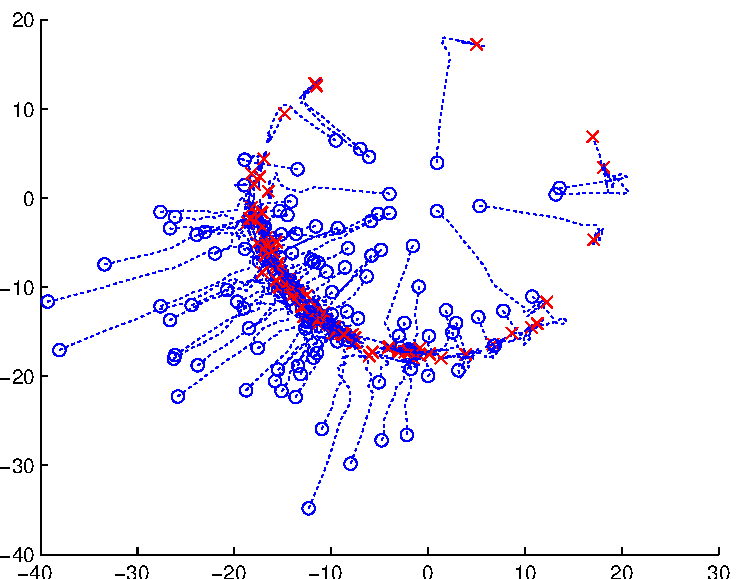
\includegraphics[width=0.45\columnwidth]{nlng_example_frame.pdf}
\caption{An example of the S-CPPF particle motion running on the multivariate benchmark model, showing $2$ of $10$ state dimensions. Prior states are shown with circles and posterior states with crosses.}
\label{fig:nlng_example_frame}
\end{figure}



\subsection{A Difficult Tracking Problem}

Now to a more applied problem. We consider tracking a small aircraft over a mapped landscape. Time of flight and doppler measurements from a radio transmitter on the aircraft provide accurate measurements of range $\rng{\rt}$, and range rate $\rng{\rt}$, but only a low resolution measurement of bearing $\bng{\rt}$. In addition, accurate measurements are made of the height above the ground $\hei{\rt}$. The profile of the terrain (i.e. the height of the ground above a datum at each point) has been mapped.

At $\rt$, the latent state for our model is,
%
\begin{IEEEeqnarray}{rCl}
 \ls{\rt} & = & \begin{bmatrix} \pos{\rt} \\ \vel{\rt} \end{bmatrix} \nonumber      ,
\end{IEEEeqnarray}
%
where $\pos{\rt}$ and $\vel{\rt}$ are the $3$-dimensional position and velocity of the aircraft respectively, and the observation is,
%
\begin{IEEEeqnarray}{rCl}
 \ob{\rt} & = & \begin{bmatrix} \bng{\rt} \\ \rng{\rt} \\ \hei{\rt} \\ \rngrt{\rt} \end{bmatrix}       .
\end{IEEEeqnarray}
%
The observation function is described by the following equations,
%
\begin{IEEEeqnarray}{rCl}
 \bng{\rt}   & = & \arctan\left(\frac{\pos{\rt,1}}{\pos{\rt,2}}\right) \nonumber \\
 \rng{\rt}   & = & \sqrt{ \pos{\rt,1}^2 + \pos{\rt,3}^2 + \pos{\rt,3}^2 } \nonumber \\
 \hei{\rt}   & = & \pos{\rt,3} - \terrain( \pos{\rt,1}, \pos{\rt,2} ) \nonumber \\
 \rngrt{\rt} & = & \frac{ \pos{\rt}\cdot\vel{\rt} }{ \rng{\rt} } \nonumber      ,
\end{IEEEeqnarray}
%
where $\terrain( \pos{\rt,1}, \pos{\rt,2} )$ is the terrain height at the corresponding horizontal coordinates. The four measurements are independent and the respective variances are $\frac{\pi}{9}^2$, $0.1^2$, $0.1^2$, $0.1^2$.

Two linear transition models have been used, both based on a near-constant velocity model, one with a Gaussian density and one with a Student-t density with $\dof = 3$ degrees of freedom,
%
\begin{IEEEeqnarray}{rCl}
 \transfun_1(\ls{\rt} | \ls{\rt-1}) & = & \normal{\ls{\rt}}{\transmat\ls{\rt-1}}{\transcov} \nonumber \\
 \transfun_2(\ls{\rt} | \ls{\rt-1}) & = & \studentt{\ls{\rt}}{\transmat\ls{\rt-1}}{\transcov}{\dof} \nonumber      ,
\end{IEEEeqnarray}
%
\begin{IEEEeqnarray}{rCl}
 \transmat & = & \begin{bmatrix} I & I \\ 0 & I \end{bmatrix} \nonumber \\
 \transcov & = & 10 \begin{bmatrix} \frac{1}{3} I & \frac{1}{2} I \\ \frac{1}{2} I &\ I \end{bmatrix} \nonumber \\
\end{IEEEeqnarray}

The accurate measurements of range, range rate and height constrain the region of high posterior probability to lie on a $3$ dimensional subspace, which can take some unusual shapes (see figure~\ref{fig:drone_example_frame}). This again means that particle filters using simple Gaussian importance densities do not perform well. Furthermore, the optimal Gaussian importance density method performs poorly as the maximisation procedure struggles with the narrow mode. For the simulations presented here, the terrain profile was modelled as a mixture of randomly-generated Gaussian blobs. An example is shown in figure~\ref{fig:drone_terrain_map}.
%
\begin{figure}
\centering
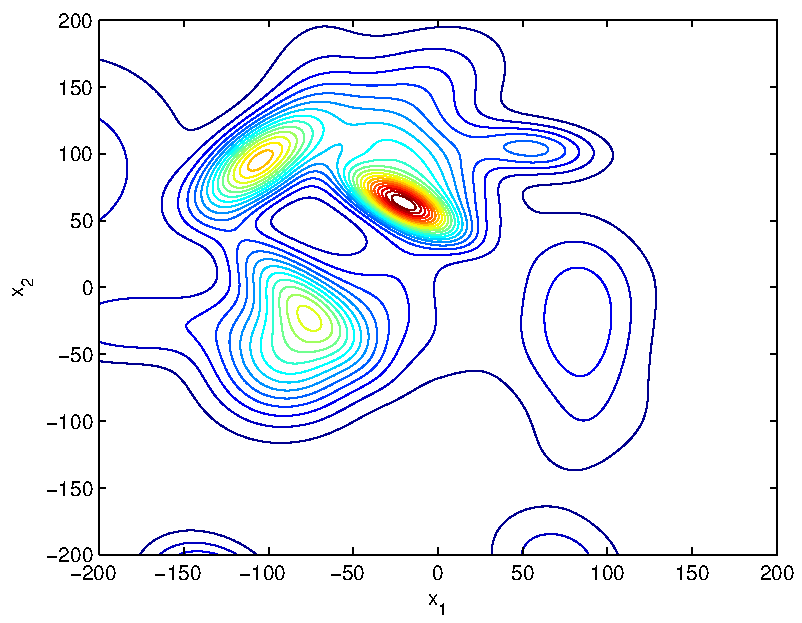
\includegraphics[width=0.45\columnwidth]{drone_terrain_map.pdf}
\caption{Contour plot of an example simulated terrain map.}
\label{fig:drone_terrain_map}
\end{figure}

The following particle filters were tested on the terrain tracking model:
\begin{itemize}
  \item A bootstrap particle filter (BPF).
  \item A particle filter using a UKF-type importance density (UPF).
  \item An optimal Gaussian importance particle filter (OGIPF).
  \item A deterministic composite proposal particle filter with $\lgexpsf=0$ (D-CPPF).
\end{itemize}

The number of particles used by each algorithm was selected so that the running times were roughly equal. The CPPF used in the region of $5$ to $10$ steps per time frame. For the student-t transition density, the CPPFs use the scale mixture of normals method.

Figure~\ref{fig:drone_example_frame} shows the motion of the particles from the stochastic CPPF on a typical frame, and the awkward shape of the posterior mode.% Figure~\ref{} shows the effective sample sizes of the particle approximations over a typical run with the Gaussian transition density.
%
\begin{figure}
\centering
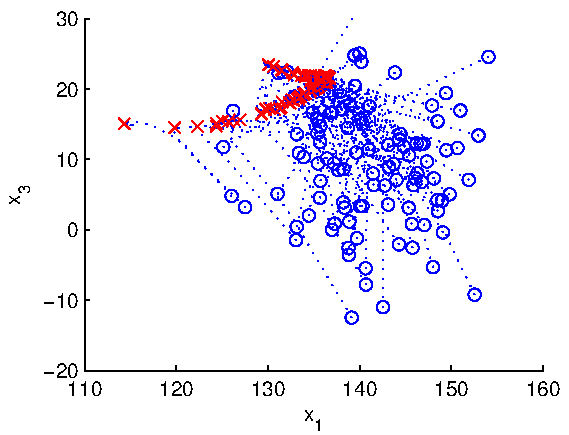
\includegraphics[width=0.45\columnwidth]{drone_example_frame.pdf}
\caption{An example of the S-CPPF particle motion running on the terrain tracking model, showing one horizontal and the vertical state component. Prior states are shown with circles and posterior states with crosses.}
\label{fig:drone_example_frame}
\end{figure}

A stochastic CPPF using resample-move was also tested, with the number of particles adjusted for a roughly-equal running time. This obtained almost identical average RMSEs to the deterministic CPPF, but higher effective sample sizes. Using $\lgexpsf=0.3$, roughly $25$--$50\%$ of the MH steps were accepted at each time step.

Table~\ref{tab:drone_results_gaussian} shows the average ESSs and RMSEs for each algorithm over 100 simulated data sets, each of 100 time steps using the Gaussian transition density. The same is shown for the student-t transition density in table~\ref{tab:drone_results_studentt}.
%
\begin{table}
\centering
\begin{tabular}{l||c|c|c}
Algorithm                                & $N_F$ & ESS  & RMSE \\
\hline
Bootstrap                                &  6000 &  1.0 & 78.6 \\
UKF Proposal                             &   460 &  2.4 & 70.2 \\
Optimal Gaussian Proposal                &    10 &  3.1 & 62.9 \\
Deterministic Composite Proposal         &   180 & 56.4 & 22.3 \\
\end{tabular}
\caption{Algorithm performance results on the terrain tracking model with Gaussian innovations.}
\label{tab:drone_results_gaussian}
\end{table}
%
\begin{table}
\centering
\begin{tabular}{l||c|c|c}
Algorithm                                & $N_F$ & ESS  & RMSE \\
\hline
Bootstrap                                &  6000 &  1.0 & 133.7 \\
UKF Proposal                             &   460 &  3.4 & 110.3 \\
Optimal Gaussian Proposal                &    10 &  2.9 & 105.1 \\
Deterministic Composite Proposal         &   180 & 17.2 & 48.0 \\
\end{tabular}
\caption{Algorithm performance results on the terrain tracking model with student-t innovations.}
\label{tab:drone_results_studentt}
\end{table}



\subsection{A Heartbeat Inference Problem}

As a final example, we consider the problem of detecting heartbeats in a vibration signal. Measurements from an accelerometer are first partitioned into segments believed to contain a heartbeat, and a particle filter is then used to infer its properties. The $t$th heartbeat is modelled parametrically as the product of a Gaussian envelope with amplitude $\amp{\rt}$ and width $\wid{\rt}$, and a sine wave carrier with frequency $\freq{\rt}$ and relative phase $\pha{\rt}$. The time shift of the centre of the heartbeat within the measurement is $\del{\rt}$, and the sensor exhibits a D.C. bias $\bias{\rt}$ which varies slowly over time. The resulting observation function is highly nonlinear, with the $d$th component given by,
%
\begin{IEEEeqnarray}{rCl}
 \obsfun(\ls{\rt})_d & = & \amp{\rt} \exp\left\{ -\frac{ (T\,d - \del{\rt})^2 }{ 2\wid{\rt}^2 } \right\} \sin\left( \freq{\rt}(T\,d - \del{\rt}) + \pha{\rt} \right) + \bias{\rt} \nonumber      ,
\end{IEEEeqnarray}
%
where $T$ is the sampling period of the sensor. Each observation consists of $50$ time samples and the observation density is modelled as a Gaussian with a covariance matrix $0.2^2 I$. An example heartbeat simulated from this model is shown in figure~\ref{fig:sineha_example_beat}.
%
\begin{figure}
\centering
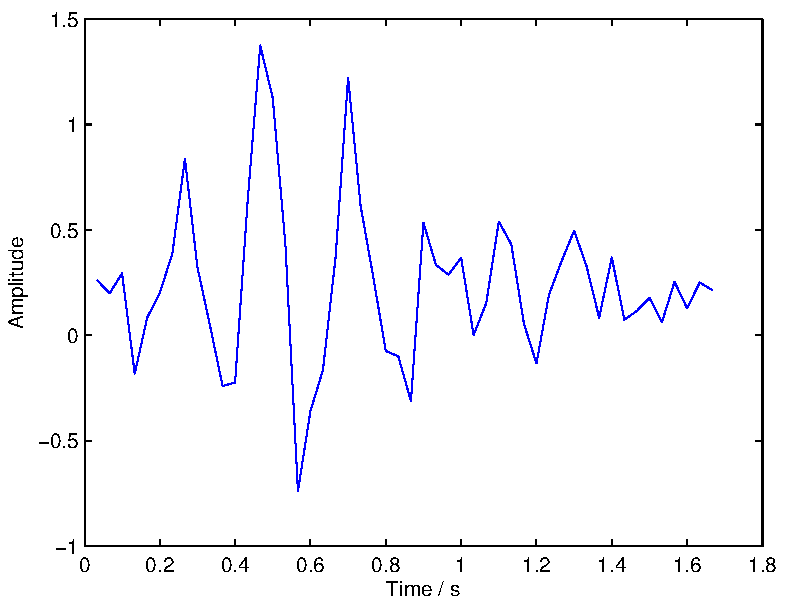
\includegraphics[width=0.45\columnwidth]{sineha_example_beat.pdf}
\caption{An example heartbeat simulated from the model.}
\label{fig:sineha_example_beat}
\end{figure}

The latent state is,
%
\begin{IEEEeqnarray}{rCl}
 \ls{\rt} & = & \begin{bmatrix} \amp{\rt} & \wid{\rt} & \del{\rt} & \freq{\rt} & \pha{\rt} & \bias{\rt} \end{bmatrix}^T      .
\end{IEEEeqnarray}
%
The transition density is factorised into independent terms, with $\freq{\rt}$, $\pha{\rt}$ and $\bias{\rt}$ evolving according to a Gaussian random walk, and $\wid{\rt}$ according to a geometric random walk (i.e. with a log-normal density), while $\del{\rt}$ and $\amp{\rt}$ are gamma distributed with no dependence on their past values.
%
%\begin{IEEEeqnarray}{rCl}
% p(\amp{\rt} )                & = & \gammaden{\amp{\rt}-0.5}{10}{0.05} \nonumber \\
% p(\wid{\rt} | \wid{\rt-1})   & = & \lognormal{\wid{\rt}}{}{} \nonumber \\
% p(\del{\rt})                 & = &   \nonumber \\
% p(\freq{\rt} | \freq{\rt-1}) & = &   \nonumber \\
% p(\pha{\rt} | \pha{\rt-1})   & = &   \nonumber \\
% p(\bias{\rt} | \bias{\rt-1}) & = &   \nonumber      ,
%\end{IEEEeqnarray}
%%
%where {\meta PARAMETERS}.

The complications introduced in the posterior distribution by the highly multi-modal observation density mean that simple Gaussian importance densities do not work very well. Particle filters using extended or unscented Kalman-type importance densities fail immediately on this model.

In order to use a CPPF with this model, the OID density sequence must be approximated with Gaussians. This is achieved by linearising the observation model around the current state \eqref{eg:linearised_Gaussian_approx} and using the log-density Taylor series truncation method for the prior \eqref{eg:general_Gaussian_approx}. The variance terms in this latter approximation are limited to be no greater than the prior variances. The CPPF used in the region of $5$ to $15$ steps per time frame, with the exception of a few particles which tended to ``get stuck'' and were discarded after 50 steps.

The following particle filters were tested on the heartbeat inference model:
\begin{itemize}
  \item A bootstrap particle filter (BPF)
  \item An optimal Gaussian importance particle filter (OGIPF).
  \item A deterministic composite proposal particle filter with $\lgexpsf=0$ (D-CPPF).
\end{itemize}

The number of particles used by each algorithm was selected so that the running times were roughly equal. The CPPFs both use the adaptive step size method. Figure~\ref{fig:sineha_example_frame} shows the motion of the particles from the deterministic CPPF on a typical frame. Table~\ref{tab:sineha_results} shows the average ESSs and RMSEs for each algorithm over 100 simulated data sets, each of 100 time steps.%Figure~\ref{} shows the effective sample sizes of the particle approximations over a typical run.
%
\begin{table}
\centering
\begin{tabular}{l||c|c|c}
Algorithm                                & $N_F$ & ESS  & RMSE \\
\hline
Bootstrap                                & 15000 &  7.6 &  2.0 \\
Optimal Gaussian Proposal                &   200 &  8.8 &  2.0 \\
Deterministic Composite Proposal         &   800 & 72.8 &  1.4 \\
\end{tabular}
\caption{Algorithm performance results on the heartbeat inference model.}
\label{tab:sineha_results}
\end{table}
%
\begin{figure}
\centering
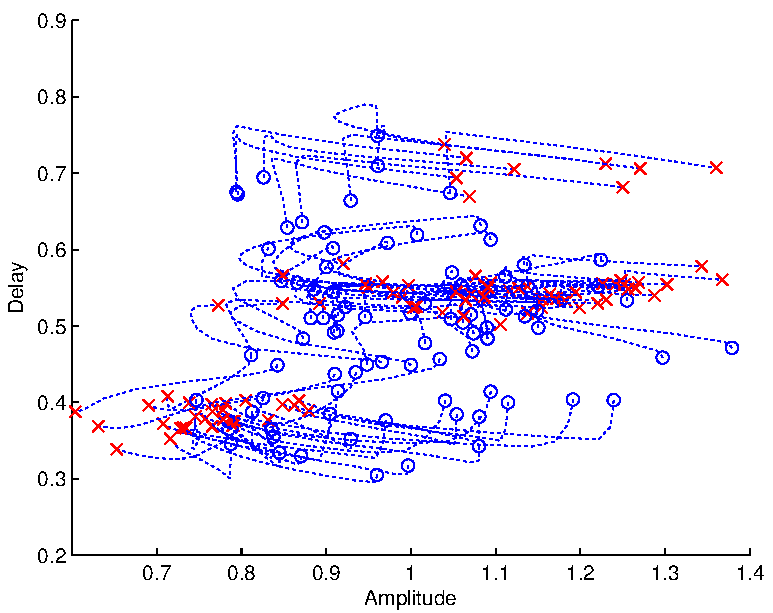
\includegraphics[width=0.45\columnwidth]{sineha_example_frame.pdf}
\caption{An example of the S-CPPF particle motion running on the heartbeat inference model, showing amplitude and delay state components. Prior states are shown with circles and posterior states with crosses.}
\label{fig:sineha_example_frame}
\end{figure}


\section{Conclusions}

\section{THINGS TO DO}
\begin{itemize}
  \item Add conclusions
  \item Add abstract
\end{itemize}



\appendix

\section{Proof of Lemma~\ref{lem:state_SDE}: A Stochastic Differential Equation For State Evolution} \label{app:state_SDE}

For clarity, write $\lgoimean{\pt}$ instead of $\lgoimeanapprox{\pt}{\ls{\pt_0}}$ and $\lgoicov{\pt}$ instead of $\lgoicovapprox{\pt}{\ls{\pt_0}}$ throughout this proof.

From \eqref{eq:state_update}, the state update for a short interval of pseudo-time is,
%
\begin{IEEEeqnarray}{rCl}
 \ls{\pt+\dpt} & = & \lgoimean{\pt+\dpt} + \lgupdmeanmat{\pt,\pt+\dpt}(\ls{\pt}-\lgoimean{\pt}) + \lgupdcov{\pt,\pt+\dpt}^{\half} \stdnorm{\Delta} \nonumber \\
 \lgupdmeanmat{\pt,\pt+\dpt} & = & \exp\left\{-\half\lgexpsf\dpt\right\} \lgoicov{\pt+\dpt}^{\half}\lgoicov{\pt}^{-\half} \nonumber \\
 \lgupdcov{\pt,\pt+\dpt} & = & \left[1-\exp\left\{-\lgexpsf\dpt\right\}\right]\lgoicov{\pt+\dpt} \nonumber         .
\end{IEEEeqnarray}

For small intervals,
%
\begin{IEEEeqnarray}{rCl}
 \exp\left\{-\half\lgexpsf\dpt\right\} & = & 1 - \half\lgexpsf\dpt + \bigo{\dpt^2} \nonumber \\
 \lgoimean{\pt+\dpt}                   & = & \lgoimean{\pt} + \dpt \frac{\partial \lgoimean{\pt}}{\partial \pt} + \bigo{\dpt^2} \nonumber \\
 \lgoicov{\pt+\dpt}                    & = & \lgoicov{\pt}  + \dpt \frac{\partial \lgoicov{\pt} }{\partial \pt} + \bigo{\dpt^2} \nonumber \\
                                       & = & \left[ I + \dpt \frac{\partial \lgoicov{\pt} }{\partial \pt} \lgoicov{\pt}^{-1} \right] \lgoicov{\pt} + \bigo{\dpt^2} \nonumber \\
 \lgoicov{\pt+\dpt}^{\half}            & = & \left[ I + \half \dpt \frac{\partial \lgoicov{\pt} }{\partial \pt} \lgoicov{\pt}^{-1} \right] \lgoicov{\pt}^{\half} + \bigo{\dpt^2} \nonumber      .
\end{IEEEeqnarray}
%
Hence,
%
\begin{IEEEeqnarray}{rCl}
 \ls{\pt+\dpt} - \ls{\pt} & = & \lgoimean{\pt} + \dpt \frac{\partial \lgoimean{\pt}}{\partial \pt} + \left(1 - \half\lgexpsf\dpt + \bigo{\dpt^2}\right) \left( I + \half \dpt \frac{\partial \lgoicov{\pt} }{\partial \pt} \lgoicov{\pt}^{-1} \right)(\ls{\pt}-\lgoimean{\pt}) \nonumber \\
 &   & \qquad \qquad + \: \dpt^{\half} \lgexpsf^{\half} \left( I + \half \dpt \frac{\partial \lgoicov{\pt} }{\partial \pt} \lgoicov{\pt}^{-1} \right) \lgoicov{\pt}^{\half} \stdnorm{\Delta} + \bigo{\dpt^2} - \ls{\pt} \nonumber \\
  & = & \left[ \frac{\partial \lgoimean{\pt}}{\partial \pt} + \half \left( \frac{\partial \lgoicov{\pt} }{\partial \pt} \lgoicov{\pt}^{-1} - \lgexpsf I \right) (\ls{\pt}-\lgoimean{\pt}) \right] \dpt + \lgexpsf^{\half} \lgoicov{\pt}^{\half} \dpt^{\half} \stdnorm{\Delta} + \bigo{\dpt^2} \nonumber      .
\end{IEEEeqnarray}
%
In the limit $\dpt\rightarrow0$, this becomes a stochastic differential equation,
%
\begin{IEEEeqnarray}{rCl}
 d\ls{\pt} & = & \left[ \frac{\partial \lgoimean{\pt}}{\partial \pt} + \half \left( \frac{\partial \lgoicov{\pt} }{\partial \pt} \lgoicov{\pt}^{-1} - \lgexpsf I \right) (\ls{\pt}-\lgoimean{\pt}) \right] d\pt + \lgexpsf^{\half} \lgoicov{\pt}^{\half} d\lginfbm{\pt}      ,
\end{IEEEeqnarray}
%
where $\lginfbm{\pt}$ is a standard Brownian motion process.

When the OID is, or is approximated by, a Gaussian with moments,
%
\begin{IEEEeqnarray}{rCl}
 \lgoicov{\pt} & = & \left[ \transcov^{-1} + \pt \obsmat^T \obscov^{-1} \obsmat \right]^{-1} \nonumber \\
 \lgoimean{\pt}    & = & \lgoicov{\pt} \left[ \transcov^{-1} \transfun(\ls{\rt-1}) + \pt \obsmat^T \obscov^{-1} \ob{\rt} \right] \nonumber     .
\end{IEEEeqnarray}
%
then
%
\begin{IEEEeqnarray}{rCl}
 \frac{\partial \lgoicov{\pt} }{\partial \pt} & = & -\lgoicov{\pt} \obsmat^T \obscov^{-1} \obsmat \lgoicov{\pt} \nonumber \\
 \frac{\partial \lgoimean{\pt}}{\partial \pt} & = & \lgoicov{\pt} \obsmat^T \obscov^{-1}(\ob{\rt}-\obsmat\lgoimean{\pt}) \nonumber       ,
\end{IEEEeqnarray}
%
and the state evolution stochastic differential equation is,
%
\begin{IEEEeqnarray}{rCl}
 d\ls{\pt} & = & \left[ \lgoicov{\pt} \obsmat^T \obscov^{-1} \left( (\ob{\rt}-\obsmat\lgoimean{\pt}) - \half \obsmat (\ls{\pt}-\lgoimean{\pt}) \right) - \half \lgexpsf (\ls{\pt}-\lgoimean{\pt}) \right] d\pt + \lgexpsf^{\half} \lgoicov{\pt}^{\half} d\lginfbm{\pt} \nonumber       .
\end{IEEEeqnarray}



\bibliographystyle{chicago}
\bibliography{D:/pb404/Dropbox/PhD/OTbib}
%\bibliography{/home/pete/Dropbox/PhD/OTbib}

\end{document} 